\documentclass{beamer}
\usepackage[latin1]{inputenc}
\usetheme{Warsaw}

\title[TagFS]{A tag based filesystem}
\author{Catalina Macalet, Eugen Hristev, Mihai Dinu, Sorin Dumitru}
\institute{Politehnic University of Bucharest}
\date{Nov 11, 2010}

\begin{document}

\begin{frame}
  \titlepage
\end{frame}

\section{Introduction}

\begin{frame}{Introduction}
\end{frame}

\section{Architecture}

\begin{frame}
  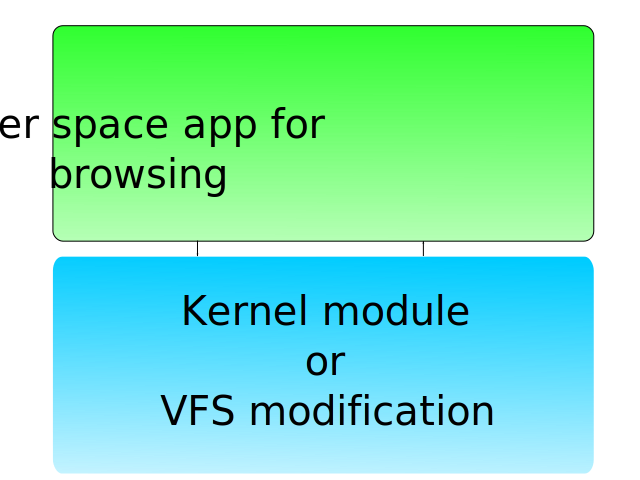
\includegraphics[scale=0.6]{art/archall.pdf}
\end{frame}

\begin{frame}
  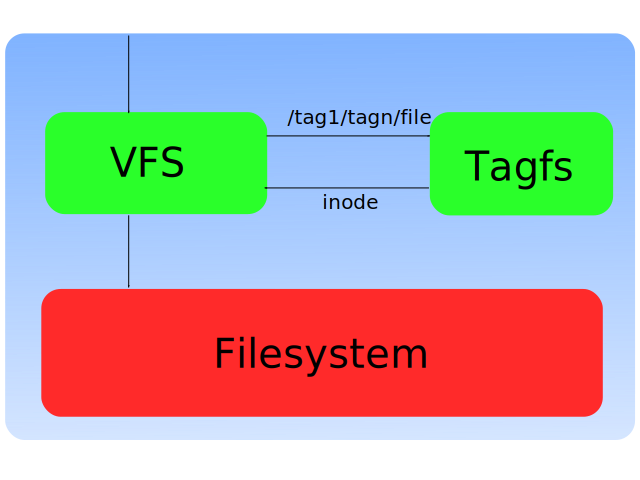
\includegraphics[scale=0.6]{art/archdetail.pdf}
\end{frame}

\section{Related work}

\begin{frame}
  
  \begin{itemize}
  \item TagFS: Bringing Semantic Metadata to the Filesystem
    \begin{itemize}
    \item \url{http://www.eswc2006.org/poster-papers/FP31-Schenk.pdf}
    \end{itemize}
    
  \item Nepomuk
    \begin{itemize}
    \item \url{http://nepomuk.semanticdesktop.org/xwiki/bin/view/Main1/Deliverables}
    \end{itemize}
    
  \item Keywords: metadata, database
  \end{itemize}
  
\end{frame}

\section{Current status}

\begin{frame}{Current status}
  \begin{itemize}
  \item Studied related work
  \item Stated expected behaviour
    \begin{itemize}
    \item Picture or a couple of cmds outpur
    \end{itemize}
  \item Identified pros and cons for the two possible solutions
    \begin{itemize}
    \item maybe listing a couple of + - for every solution,maybe we
      can make 2 slides out of this
    \end{itemize}
  \end{itemize}
\end{frame}

\section{Employed Technologies}

\begin{frame}
  \begin{itemize}
  \item Ubuntu 10.10:
	\begin{itemize}  
	\item freeware  source code is free for all and can be modified to suite demands
	\item latest kernel version - 2.6.35 
	\item stable workspace
	\end{itemize}
  \item GCC 4.4.5:
	\begin{itemize} 	
	\item latest C compiler
	\item freeware
	\end{itemize}
  \item Eclipse IDE
  \end{itemize}
\end{frame}

\begin{frame}
  \begin{itemize}
  \item FUSE  Filesystem in USErspace
	\begin{itemize}
	\item implement fully functional filesystem in a userspace program 
	\item piece of code that communicates with the kernel as a filesystem would
	\item runs on Linux kernels 2.4.X and 2.6.X
    \item libfuse - http://fuse.sourceforge.net/
    \end{itemize}
  \item C programming language
  \end{itemize}
\end{frame}

\section{Short term planning}

\begin{frame}
  \begin{itemize}
    \item Determine if VFS implementation is feasible
    \item Data organization
    \item Start coding
  \end{itemize}
\end{frame}

\end{document}
